\documentclass[tikz,border=5pt]{standalone}
\usepackage{pgfplots}
\pgfplotsset{compat=1.18}
\begin{document}
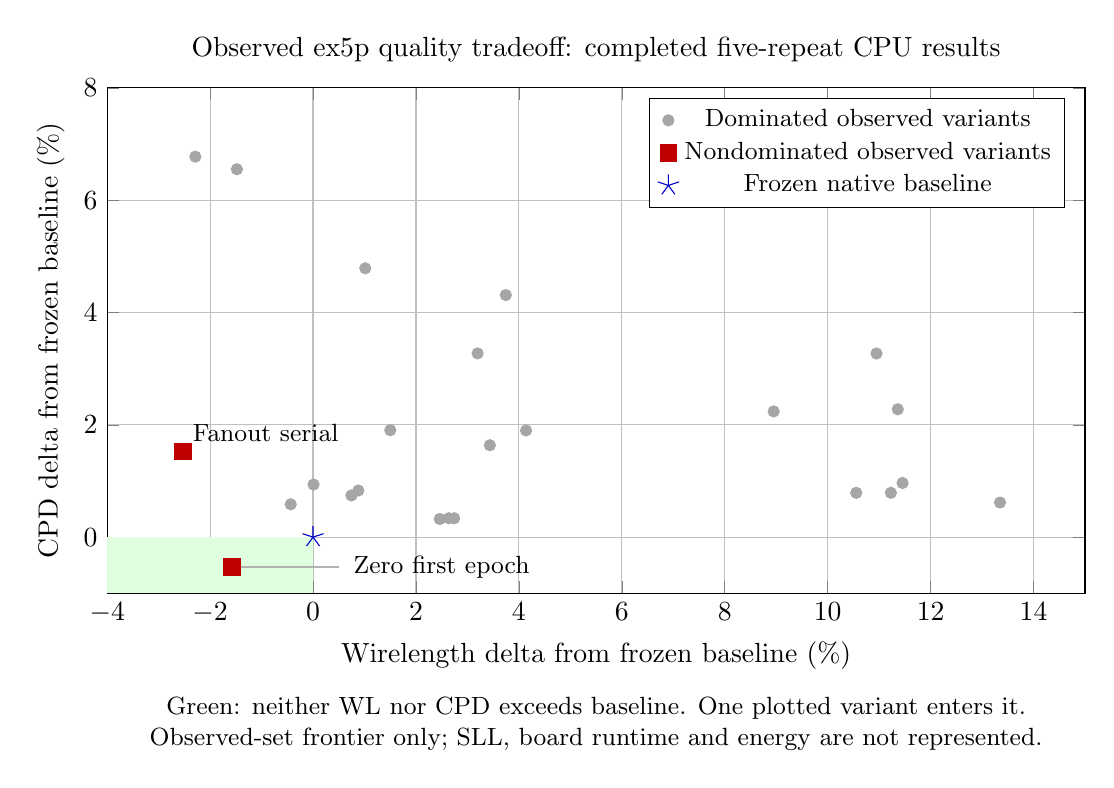
\begin{tikzpicture}
\begin{axis}[width=14cm,height=8cm,xmin=-4,xmax=15,ymin=-1,ymax=8,
xlabel={Wirelength delta from frozen baseline (\%)},
ylabel={CPD delta from frozen baseline (\%)},grid=major,
title={Observed ex5p quality tradeoff: completed five-repeat CPU results},
legend style={at={(0.98,0.98)},anchor=north east,font=\small}]
\fill[green!12] (axis cs:-4,-1) rectangle (axis cs:0,0);
\addplot[gray!70,only marks,mark=*,mark size=2pt] coordinates {(-2.286837748,6.775051378) (-1.479718543,6.551101676) (-0.434602649,0.584248315) (0.010347682,0.936005591) (0.745033113,0.741950571) (0.879552980,0.829759686) (1.014072848,4.787627977) (1.500413907,1.904093280) (2.462748344,0.322175083) (2.638658940,0.336028716) (2.742135762,0.336028716) (3.197433775,3.271644739) (3.435430464,1.636082776) (3.745860927,4.310563030) (4.139072848,1.898780984) (8.950745033,2.238455393) (10.554635762,0.788615439) (10.947847682,3.269873974) (11.227235099,0.788615439) (11.361754967,2.276578924) (11.454884106,0.963504532) (13.348509934,0.615497111)};
\addlegendentry{Dominated observed variants}
\addplot[red!75!black,only marks,mark=square*,mark size=3pt] coordinates {(-2.524834437,1.525357877) (-1.572847682,-0.531854501)};
\addlegendentry{Nondominated observed variants}
\addplot[blue!80!black,only marks,mark=star,mark size=4pt] coordinates {(0,0)};
\addlegendentry{Frozen native baseline}
\node[font=\small,anchor=south west] at (axis cs:-2.524834437,1.525357876) {Fanout serial};
\draw[gray!60] (axis cs:-1.572847682,-0.531854501) -- (axis cs:0.5,-0.531854501);
\node[font=\small,anchor=west] at (axis cs:0.6,-0.531854501) {Zero first epoch};
\end{axis}
\node[align=center,font=\small,anchor=north] at ([yshift=-1.2cm]current axis.south)
{Green: neither WL nor CPD exceeds baseline. One plotted variant enters it.\\
Observed-set frontier only; SLL, board runtime and energy are not represented.};
\end{tikzpicture}
\end{document}
